\documentclass[sigconf,anonymous]{acmart}
\usepackage{amsmath}

% Visible draft marker; replace each occurrence with a verified \cite{...}.
\newcommand{\citationneeded}{\textit{[citation needed]}}

\AtBeginDocument{%
  \providecommand\BibTeX{{Bib\TeX}}}

\begin{document}

\title{CipherStore: A Computational Storage Architecture for FPGA-Accelerated FHE Ciphertext Generation}

\author{Anonymous Author(s)}

\begin{abstract}
Fully Homomorphic Encryption (FHE) enables computation directly on encrypted data, but its high computational and data overheads remain a major barrier to practical deployment. Existing research has primarily focused on accelerating ciphertext computation, while \textbf{ciphertext generation} is still commonly treated as a host-side preprocessing step. For large inputs, ciphertext generation incurs non-trivial cryptographic computation and significant ciphertext expansion, leading to increased host CPU usage, memory buffering, and subsequent data-movement overhead. Meanwhile, existing hardware acceleration efforts for encryption and decryption mainly optimize individual cryptographic kernels, without systematically organizing the complete execution path from persistent data to computation-ready ciphertexts or providing an application abstraction for this process.

This paper presents \textbf{CipherStore}, a computational storage architecture for FPGA-accelerated FHE ciphertext generation. CipherStore moves ciphertext generation close to persistent data and combines FPGA-accelerated encryption with storage-side data processing to construct a near-storage execution path from data access and preprocessing to ciphertext generation. We further introduce a computational-storage application model that maps application-level data access, processing, and encryption requirements to device-side tasks. We instantiate CipherStore with TFHE and implement a prototype on a SoC-FPGA computational storage device using HLS-based hardware operators. For a 4~KB u8 workload, the FPGA implementation achieves a \textbf{5.33$\times$ speedup} in TFHE encryption over host-CPU generation, while the complete ciphertext-generation path improves end-to-end latency by \textbf{3.26$\times$} and reduces host-side CPU time by \textbf{91.8\%}. Ciphertexts generated by CipherStore are also directly consumable by an existing FHE computing backend and successfully support downstream homomorphic computation.
\end{abstract}

\keywords{fully homomorphic encryption, TFHE, LWE, FPGA, computational storage}

\maketitle

% Allow modest extra flexibility when breaking long English lines in two columns.
\begingroup
\setlength{\emergencystretch}{1em}
\section{Introduction}
\label{sec:introduction}
Fully homomorphic encryption (FHE) enables computation directly on encrypted data without requiring decryption, making it a promising foundation for privacy-preserving remote computing. Its practical adoption, however, remains constrained by computation and data overheads that are substantially higher than those of plaintext processing. Recent studies have therefore explored GPUs, FPGAs, and ASICs to accelerate the core operations of FHE. Architectures such as F1, BTS, and CraterLake have demonstrated that specialized hardware can substantially improve the performance of both FHE primitives and complete encrypted programs~\cite{f1,bts,craterlake}.

An end-to-end FHE workflow, however, involves more than ciphertext computation. Any data involved in subsequent homomorphic computation must first undergo ciphertext generation, which transforms source data into the corresponding FHE ciphertexts. Accelerating back-end ciphertext computation does not eliminate this front-end process. For large datasets, ciphertext generation not only performs nontrivial cryptographic computation but also produces representations substantially larger than the original plaintext. Consequently, it continuously consumes host computing resources while increasing memory footprint, buffering requirements, and the cost of subsequent data movement. Prior FHE system studies have identified large ciphertext volumes as an important source of memory and data-movement overhead~\cite{f1,craterlake,hera}. Meanwhile, an FPGA implementation of LWE/TFHE encryption and decryption has shown that ciphertext generation itself offers opportunities for hardware acceleration~\cite{feryputri-lwe-fpga}. As ciphertext computation becomes increasingly accelerated by specialized hardware, improving the throughput of ciphertext generation while reducing its sustained demand on host CPU and memory resources becomes a distinct end-to-end systems problem.

Existing work has not yet treated FHE ciphertext generation as a complete systems problem. On the hardware side, prior studies have demonstrated the potential of accelerating FHE encryption and decryption, but they have focused primarily on the implementation and performance of individual cryptographic kernels. In practical systems, however, ciphertext generation is not an isolated cryptographic operation. In data-driven applications, the source data typically reside in persistent objects such as files, tables, or records. Transforming these objects into ciphertexts that can be consumed by an FHE back end requires a complete path that includes data access, application-specific preprocessing, and cryptographic generation. How to organize this path efficiently around persistent data therefore remains an architectural question.

On the software side, existing FHE stacks generally expose encryption as an operation over plaintext objects that have already been prepared in memory, implicitly assuming that data retrieval and preprocessing are handled by the application beforehand. \citationneeded{} Although this abstraction is suitable for conventional memory-resident workflows, it does not directly capture ciphertext-generation tasks over persistent data. When the target data remain in storage, an application must specify which data should be processed, what preprocessing should be performed, and how the resulting values should be converted into ciphertexts. FHE ciphertext generation therefore requires not only an appropriate compute architecture but also an application model that connects high-level data requirements to the underlying storage access, preprocessing, and encryption operations.

Computational storage (CS) provides a natural design point for addressing these requirements. By placing computing capabilities close to stored data, CS enables selected operations to execute on the storage side, thereby reducing host processing and data-movement overheads. Database analytics, compression, conventional encryption, and encoding have all been studied as representative computational-storage workloads. \citationneeded{} In an FHE system, this model allows ciphertext generation to be elevated from host-side preprocessing to a storage-side service. An FPGA-based computational storage device (CSD) can accelerate ciphertext generation while applying application-specific preprocessing before the data enter the encrypted domain. For data-driven FHE workloads that access only selected records or fields, the CSD can first identify the relevant data and then generate ciphertexts only for the selected values. This approach avoids encrypting irrelevant data and reduces the associated storage, buffering, and downstream processing overheads. Moreover, computational storage already provides architectural, programming-model, and API abstractions for mapping application requests to device-side computation. \citationneeded{} It therefore offers both a new execution location for TFHE ciphertext generation and a systems foundation for building a ciphertext-generation application model over persistent data.

This work uses TFHE (Fast Fully Homomorphic Encryption over the Torus) as a concrete instance of this design. TFHE is an LWE-family FHE scheme that supports fine-grained encrypted computation through bootstrapping. Its fresh encryption and decryption procedures have well-defined computational structures and are amenable to FPGA acceleration. \citationneeded{} Based on these properties, we propose a computational-storage architecture for FHE ciphertext generation and implement it for TFHE. The proposed design integrates hardware-accelerated TFHE encryption and decryption with the necessary data-processing capabilities on a CSD FPGA. We further define a computational-storage application model for ciphertext generation that connects application-level data requirements to device-side storage access, preprocessing, and encryption. Finally, we implement a prototype on a SoC-FPGA-based CSD and evaluate it through system-level experiments.

The main contributions of this work are as follows:
\begin{itemize}
  \item \textbf{A computational-storage architecture for FHE ciphertext generation.}
  We establish ciphertext generation as a first-class computational-storage capability. The architecture integrates TFHE encryption and decryption operators implemented using high-level synthesis (HLS) with data-filtering operators and the corresponding data paths on a CSD FPGA, enabling a near-storage hardware pipeline from persistent data to FHE ciphertexts.

  \item \textbf{A computational-storage application model for TFHE ciphertext generation.}
  The model maps application-level data requirements to device-side ciphertext-generation tasks. It allows applications to specify the storage-resident data to be processed together with the required preprocessing and encryption operations, which the system translates into storage access, data processing, and TFHE ciphertext generation.

  \item \textbf{A client interface and prototype system for producing TFHE ciphertexts.}
  We implement a client-side interface and an end-to-end prototype on a SoC-FPGA-based CSD. We compare the FPGA implementation with a CPU-based software implementation to evaluate ciphertext-generation performance and system overhead. We further connect the ciphertexts produced by the CSD to an existing homomorphic-computing back end, validating the correctness and practicality of the proposed architecture and application model within a complete FHE workflow.
\end{itemize}
\endgroup

% Keep line-breaking flexibility local to this section.
\begingroup
\setlength{\emergencystretch}{1em}
\section{Background}
\label{sec:background}

Ciphertext generation connects application data to the encrypted representations consumed by an FHE back end. In a TFHE-based system, its cost depends on the LWE encryption procedure and the number of ciphertexts used to represent each application value. The surrounding execution path determines how data reach the encryption engine and how the resulting ciphertexts are delivered.

\subsection{TFHE Encryption and Ciphertext Expansion}
\label{subsec:lwe-background}

TFHE uses LWE ciphertexts as one of its basic encrypted representations~\cite{tfhe}. In the discrete-torus representation used here, coefficients are $w$ bits wide and arithmetic is performed modulo $q=2^w$. An LWE ciphertext $\mathbf{c}=(\mathbf{a},b)$ comprises a mask $\mathbf{a}\in\mathbb{Z}_q^n$ and a body $b\in\mathbb{Z}_q$. Given a message $m$, an encoding scale $\Delta$, and a binary secret $\mathbf{s}\in\{0,1\}^n$, encryption samples $\mathbf{a}$ uniformly and an error $e$ from the prescribed noise distribution, then computes
\begin{equation}
b=\left(\sum_{j=0}^{n-1}a_js_j+\Delta m+e\right)\bmod q.
\label{eq:lwe-encryption}
\end{equation}
Here, $\Delta m$ is the torus encoding of $m$; the encoding scale and noise distribution are determined by the parameter set.

Decryption removes the mask--key inner product to obtain the phase
\begin{equation}
\phi=\left(b-\sum_{j=0}^{n-1}a_js_j\right)\bmod q
     =(\Delta m+e)\bmod q,
\label{eq:lwe-decryption}
\end{equation}
which is decoded to the nearest valid message encoding. Recovery succeeds when the error remains within the decoding interval. Unlike decryption, encryption must also generate the random mask and noise.

In our prototype, each LWE ciphertext encrypts one 2-bit message block. An 8-bit unsigned value $x$ is represented by four such blocks, ordered from least to most significant:
\begin{equation}
x=m_0+4m_1+16m_2+64m_3,
\qquad m_r\in\{0,1,2,3\}.
\label{eq:radix-representation}
\end{equation}
Encrypting the blocks independently produces four LWE ciphertexts for each input byte. Because each ciphertext contains $n+1$ coefficients, their combined uncompressed coefficient payload is
\begin{equation}
B_{\mathrm{raw}}=4(n+1)\frac{w}{8}\ \text{bytes}.
\label{eq:radix-cipher-size}
\end{equation}
This raw size excludes serialized metadata, transfer alignment, and allocated buffer capacity; compressed or seeded ciphertext representations may have different sizes. The expansion from one byte to four LWE ciphertexts makes output buffering and transfer bandwidth part of the ciphertext-generation cost.

\subsection{Prior TFHE Accelerators}
\label{subsec:tfhe-acceleration-background}

Much TFHE hardware work targets programmable bootstrapping, the costly step used to refresh ciphertexts during homomorphic evaluation. Ye et al. examine bootstrapping-key unrolling and customize ciphertext layout to improve FPGA data access and reuse~\cite{ye-tfhe-fpga}. MATCHA accelerates TFHE gate evaluation with a pipelined datapath and integer FFT/IFFT kernels~\cite{matcha}. FPT maps programmable bootstrapping to a fixed-point streaming FPGA pipeline, while Strix uses two-level ciphertext batching and streaming to improve bootstrapping throughput~\cite{fpt,strix}. These designs make different choices about data layout, arithmetic representation, and execution parallelism, but their datapaths accept existing ciphertexts and produce ciphertexts for further evaluation. They do not perform the initial LWE encryption of application data described in Section~\ref{subsec:lwe-background}.

The distinction persists when TFHE evaluation hardware is integrated with storage. Ohba et al. combine an NVMe SSD, an FPGA TFHE accelerator, and host middleware that communicates ciphertexts, keys, and secure-computing instructions through NVMe commands~\cite{ohba-nvme-tfhe}. Their reported acceleration centers on gate bootstrapping. This work establishes a precedent for a storage-connected TFHE execution platform, while leaving the path from stored plaintext to initial ciphertexts outside its principal optimization target.

Hardware support for that input path has been explored at the cryptographic-kernel level: Feryputri et al. implement TFHE LWE encryption and decryption on an FPGA~\cite{feryputri-lwe-fpga}. As Equation~\eqref{eq:lwe-encryption} shows, encryption generates a mask and noise and computes a mask--key inner product for every message block. Each block is a small plaintext value, but its ciphertext contains $n+1$ torus coefficients. Thus, moving encryption hardware close to persistent data also requires an execution path that identifies and reads the requested data, applies any required selection or preprocessing, and transfers the expanded ciphertexts. The encryption operator and the path that feeds and drains it are related but distinct design problems.

\subsection{Computational Storage Architecture and Programming Model}
\label{subsec:csd-background}

Computational storage integrates processing resources with or near persistent storage so that data can be processed without first moving the complete input to the host. The SNIA reference architecture distinguishes storage-integrated drives, separate computational storage processors, and storage arrays. Across these configurations, computational storage engines (CSEs) execute computational storage functions (CSFs) within execution environments, using function data memory (FDM) for data consumed or produced by those functions~\cite{sniacs}. These components provide a common vocabulary for device-side execution, data reduction, and host--device programming.

\emph{Near-storage execution.} Programmable SSD and CSD prototypes have placed application processing on embedded processors or FPGA logic within the storage system~\cite{kang-smartssd,willow,biscuit,insider}. Despite differences in hardware and runtime organization, these systems allow host-initiated functions to operate on stored data through a device-side execution path, reducing the need to materialize the full input in host memory.

\emph{Storage-side data reduction.} Database-oriented systems push predicates, filtering, selection, and projection toward stored records or columns~\cite{do-smartssd,biscuit,skyhook,upp}. When an operation discards data, executing it before host transfer can reduce both host-side processing and the amount of data returned; the benefit depends on the selectivity of the operation. In-storage processing also supports other functions, including string matching and decompression~\cite{insider}. Thus, the operations that a storage system can offload are broader than data-reducing database queries, while their effects on data movement depend on the size of their outputs.

\emph{Application-to-device programming interface.} A host needs a way to identify available functions, configure their parameters, invoke them, and specify where input data are read and results are written. The SNIA programming model separates resource discovery, function configuration, and function use; its CSF commands identify source and destination locations, while direct and indirect use models differ in how computation is associated with data access~\cite{sniacs}. Research systems expose complementary interfaces through application-defined SSD functions, host--device dataflow tasks, and file-oriented invocation~\cite{willow,biscuit,insider}. These interfaces connect application requests to storage-side execution without requiring the application to control every internal data transfer.
\par
\endgroup


\section{CipherStore: System Overview and Application Model}
\label{sec:cipherstore-overview}

CipherStore turns storage-resident records into LWE ciphertexts through a programmable CSD path. Record selection and projection precede encryption, so the number of generated ciphertexts follows the data required by the application. This section presents the system organization, the application-level task contract, and the mapping from a task to device execution.

\subsection{System Overview}
\label{subsec:cipherstore-organization}

Figure~\ref{fig:cipherstore-overview} shows the generation path. A client on the Host accepts a task describing stored records and the desired encrypted values. The SoC--FPGA CSD combines an SSD, device-side shared-memory namespaces (SLMs), and FPGA operators for selection, projection, and LWE encryption. The client configures these operators through the CSD interface, retrieves the generated ciphertexts, and can supply them to an FHE computation back end.

\begin{figure*}[t]
  \centering
  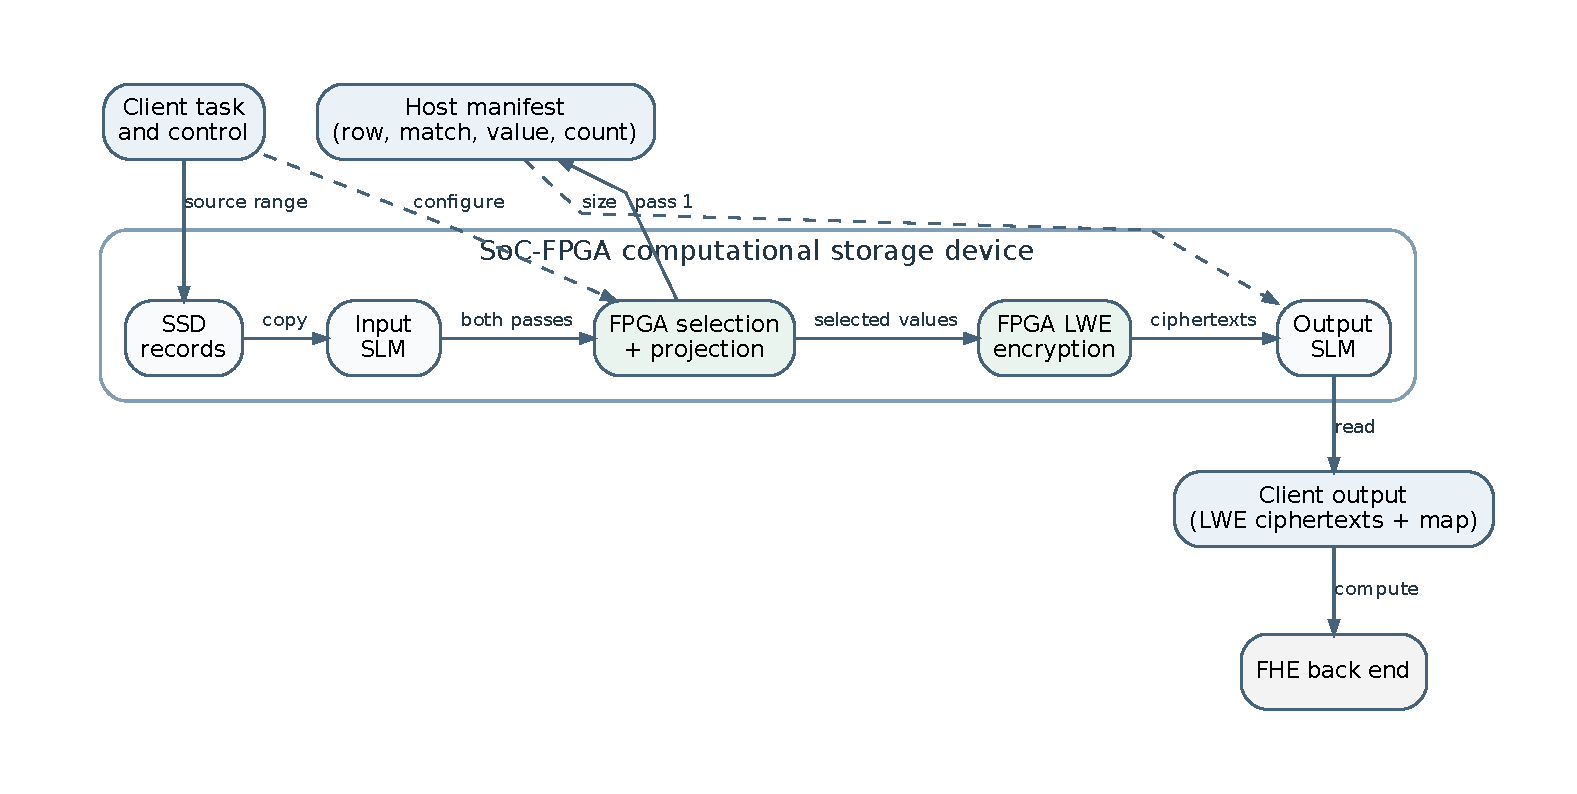
\includegraphics[width=0.94\textwidth]{../figures/system_overview.pdf}
  \Description{A client task selects records on a computational storage device. SSD records enter an input SLM. The FPGA filter returns a selection manifest in a discovery pass, then sends selected values to an LWE encryption operator in a second pass. Ciphertexts leave through an output SLM for client and optional FHE back-end use.}
  \caption{CipherStore generation path. The CSD copies source records into an input SLM, discovers the selected rows, and streams selected values through FPGA LWE encryption into an output SLM. Solid arrows carry data or selection results; dashed arrows represent client configuration and output sizing.}
  \label{fig:cipherstore-overview}
\end{figure*}

The Host manages task submission, operator contexts, and result delivery. It loads the secret key into the encryption context, while the CSD performs record selection and ciphertext generation. The discovery result returns row identities and selected projected values to the client; the subsequent generation pass emits LWE ciphertexts. The client retains the row mapping alongside the ciphertext sequence so that downstream results can be associated with their source records.

\subsection{Application Model}
\label{subsec:task-model}

CipherStore represents each request as $T=(D,Q,E,O)$: source data $D$, query $Q$, encryption configuration $E$, and output action $O$. Table~\ref{tab:cipherstore-task} maps these fields to the CSD path. The source is identified by an SSD namespace and logical block range, with a fixed-record schema defining field types and byte offsets. The query uses these fields to determine which records contribute values to encryption.

\begin{table}[H]
  \centering
  \small
  \setlength{\tabcolsep}{4pt}
  \caption{Application task fields and their execution mapping.}
  \label{tab:cipherstore-task}
  \begin{tabular}{@{}p{0.24\columnwidth}p{0.66\columnwidth}@{}}
    \toprule
    Field & Application declaration and CSD action \\
    \midrule
    Data $D$ & SSD namespace and range, record count, width, and schema; copied to the input SLM. \\
    Query $Q$ & Predicate and projected field; compiled into FPGA filter configuration. \\
    Encryption $E$ & TFHE parameter preset and key reference; configure LWE ciphertext generation. \\
    Result $O$ & Ordered ciphertexts and source-row mapping; delivered to the client or a computation back end. \\
    \midrule
    Runtime profile & Device endpoints, batch size, and transfer settings; control execution without changing task semantics. \\
    \bottomrule
  \end{tabular}
\end{table}

For records $r_0,\ldots,r_{N-1}$, let $P_Q(r_i)$ be the predicate and $\pi_Q(r_i)$ the projected value specified by $Q$. The task produces
\begin{equation}
\mathcal{C}_T=
\bigl(\operatorname{Enc}_{E}(\pi_Q(r_i))\bigr)_{i\in\mathcal{I}_Q},
\quad
\mathcal{I}_Q=(i\mid P_Q(r_i)=\mathrm{true}),
\label{eq:ciphertext-generation-task}
\end{equation}
with indices in source-record order. The companion mapping $\mathcal{I}_Q$ identifies the source record of each ciphertext after filtering. In the TFHE instantiation used here, the projected value is an unsigned byte encoded as four two-bit LWE ciphertext blocks, as described in Section~\ref{subsec:lwe-background}. Predicate evaluation can use the integer fields specified by the record schema.

The task specifies which values become ciphertexts; a separate runtime profile selects batch and transport parameters. The client validates the task and divides its source range into LBA-aligned batches. A global record offset attached to each batch preserves the mapping between generated ciphertexts and source records across the complete task.

\subsection{Mapping Tasks to Device Execution}
\label{subsec:cipherstore-execution}

For each batch, the client copies the corresponding SSD blocks into an input SLM. It then invokes the FPGA filter in discovery mode. This pass produces a deterministic-size manifest with one 64-byte entry per record and a 64-byte summary. Each entry reports its row index and match result; for a matched row it also carries the projected value. The Host obtains the selected count from the device-generated summary and uses it to configure the ciphertext output range.

The client next runs a filter--encryption program on the same input SLM. The filter streams the selected values directly to the LWE encryption operator, which writes the resulting ciphertexts to an output SLM. Thus, selection controls both the amount of cryptographic work and the size of the ciphertext result. The Host reads the output and associates its ordered ciphertexts with the row mapping from discovery. If a batch selects no records, no encryption program is issued.

The application can consume the generated LWE ciphertexts directly or pass them to a homomorphic-computation back end. In the latter workflow, returned ciphertext results can be decrypted by the CSD and applied to the selected source-row positions. Generation and downstream computation are connected by the same ciphertext sequence and row mapping defined in Equation~\eqref{eq:ciphertext-generation-task}.


\section{Integration with SoC-FPGA Computational Storage}
% 第四章：CSD集成

\subsection{System Overview}

\subsection{Host Interface and Device Runtime}

\subsection{SLM-Based Data Management}

\subsection{Task Execution and Completion}

\subsection{End-to-End Protected Data Path}

\section{Evaluation}
% 第五章：实验

\subsection{Experimental Setup}

\subsection{Correctness}

\subsection{FPGA Performance and Resource Utilization}

\subsection{Comparison with CPU and Prior Hardware}

\subsection{CSD Stage Breakdown}

\subsection{End-to-End Application}

\section{Related Work}

\subsection{TFHE Bootstrapping Accelerators}

\subsection{LWE Encryption and Decryption Hardware}

\subsection{FPGA Computational Storage}

\section{Conclusion}

\bibliographystyle{ACM-Reference-Format}
\bibliography{references}
\end{document}
